\documentclass[conference]{IEEEtran}

\IEEEoverridecommandlockouts

\usepackage[utf8]{inputenc}
\usepackage[T1]{fontenc}
\usepackage{cite}

\ifCLASSINFOpdf
  \usepackage[pdftex]{graphicx}
\else

\fi

\usepackage[cmex10]{amsmath}

\usepackage{multirow}
\usepackage{array}
\usepackage[lofdepth,lotdepth]{subfig}
\usepackage{color}
\usepackage{tabto}

\usepackage{amssymb}
\usepackage{booktabs}
\usepackage{multirow}
\usepackage{rotating}
\usepackage{amsmath}
\usepackage{algorithm}
\usepackage{algpseudocode}
\usepackage{lineno,hyperref}
\usepackage{graphicx}
\usepackage{pdflscape}
\usepackage[none]{hyphenat}

\begin{document}

\IEEEpubid{\makebox[\columnwidth]{\hfill} \hspace{\columnsep}\makebox[\columnwidth]{}}

\title{Makine Öğrenmesi Algoritmaları ile İkinci El Araç Fiyat Tahmini
\\
\*

Used Car Price Prediction with Machine Learning Algorithms
}
\author{
	
\IEEEauthorblockN{Samed ZIRHLIOĞLU}
\IEEEauthorblockA{Bilgisayar Mühendisliği\\
	18110131037\\
	Kahramanmaraş Sütçü İmam Üniversitesi\\
	Kahramanmaraş, Türkiye\\
	zirhlioglusamed@gmail.com
	}
\and
\IEEEauthorblockN{Mehtap ÖKLÜ}
\IEEEauthorblockA{Bilgisayar Mühendisliği\\
	17110131052\\
	Kahramanmaraş Sütçü İmam Üniversitesi\\
	Kahramanmaraş, Türkiye\\
	mehtap\_oklu\_06@hotmail.com
	}
}
\maketitle
\thispagestyle{plain}
\pagestyle{plain}
\begin{ozet}
Teknolojinin çok hızlı ilerlemesine bağlı olarak otomotiv sektörü de hızlı bir şekilde gelişmektedir. Bundan kaynaklı olarak artan üretim çeşitliliği, ikinci el piyasasında da büyük etki bırakmaktadır. İkinci el piyasası aktörlerinin araç alım ve satışlarında piyasanın durumunu iyi anlayarak buna göre araç ve fiyat tespitlerini yapmaları çok önem arz etmektedir. Otomotiv sektörü yolcu ve yük taşıma amaçlarına bağlı olarak birçok ana ve alt başlıkta üretim yapmaktadır. Yapılacak çalışmamızda kişisel kullanıma yönelik BMW markası gibi özgün bir otomobil markası üzerinden modelleme yapılacaktır. BMW firması her yıl farklı teknik, donanım ve dizayn özelliklerde yeni model araçları üretmektedir. Bu markaya ait araçların özellikleri (model, yıl, motor, şanzıman, Km./Mil, yakıt tipi, vergi, yakıt tüketimi, fiyat vb.) incelenerek aracın değeri tahmin edilebilir. Yapay zekâ algoritmaları (Karar Ağacı, Gradient Boost, XGB, Rastgele Orman Ağacı, LightGBM, CatBoost) kullanılarak bu değerler incelenmiştir. Projedeki sorunun tipinden dolayı regresyon algoritmalarına yer verilmiştir. Bunun nedeni ise elimizdeki bağımsız değişkenlerden hareketle, yeni bir bağımlı değişken elde etmek istememizdir.
\end{ozet}

\begin{IEEEanahtar}
Araç, Araç Özellikleri, Karar Ağacı, Gradient Boost, XGB, Rastgele Orman Ağacı, LightGBM, CatBoost
\end{IEEEanahtar}

\begin{abstract}
Depending on the rapid progress of technology, the automotive industry is also developing rapidly. Due to this, the increasing variety of production also has a great impact on the second-hand market. It is very important for the second-hand market actors to understand the situation of the market in vehicle purchases and sales and to determine the vehicle and price accordingly. The automotive sector produces in many main and sub-titles depending on the purposes of passenger and cargo transportation. In our study, modeling will be done on a unique automobile brand such as BMW brand for personal use. Every year, BMW company produces new model vehicles with different technical, equipment and design features. The value of the vehicle can be estimated by examining the characteristics of the vehicles of this brand (model, year, engine, transmission, Km./Mile, fuel type, tax, fuel consumption, price, etc.). These values were examined using artificial intelligence algorithms (Decision Tree, Gradient Boost, XGB, Random Forest Tree, LightGBM, CatBoost). Regression algorithms are included due to the type of problem in the project. The reason for this is that we want to obtain a new dependent variable based on the independent variables we have.
\end{abstract}

\begin{IEEEkeywords}
Car, Car Properties, Value, Decision Tree, Gradient Boost, XGB, Random Forest Tree, LightGBM, CatBoost
\end{IEEEkeywords}

\section{\textbf{GİRİŞ}}
\quad Ulaşım, insanlık tarihinin başlangıcından günümüze kadar, insan hayatının en temel ihtiyaçlarından birisi olmuştur. Arabalar icat edilmeden önce ulaşım; at, eşek ve deve gibi hayvanlar kullanılarak sağlanmıştır. Bu durum hem zaman hem de emek kaybına neden olmuştur.

\quad Artan dünya nüfusu ve ihtiyaçlar doğrultusunda ulaşım çok büyük bir önem kazanmıştır. Bu ihtiyaçları gidermek ve ulaşımı daha kolay hale getirmek için yapılan çalışmalar hız kazanmıştır. Bu çalışmalar sonucunda insanlar ihtiyaçları doğrultusunda tarım ve ulaşım araçlarını geliştirmiştir. Günümüzde de insanların daha konforlu ve keyifli bir ulaşım deneyimi yaşayabilmesi için bu çalışmalar devam etmektedir.

\quad Günümüzde otomobil sektörü, insanlık tarihinin en yaygın sektörlerinden ve yatırım yapılan iş kollarından birisi olmuştur. Başlangıçta sadece ulaşım ve ticaret amaçlı kullanılan otomobiller, günümüzde lüks ve ihtişamlı yaşamın sembolü haline gelmiştir\cite{1}.

\quad Arabalar uzun ömürlü araçlar oldukları için sürekli alınıp satılabilir. İkinci el olarak satılan araçların makul bir şekilde fiyatlandırılması gerekmektedir. İkinci el bir aracın makul fiyat tahmininin yapılması zor olduğu için doğru fiyatı belirleyecek bir tahmin mekanizmasına ihtiyaç duyulmaktadır\cite{2}. Bu makalede yapay zekâ kullanarak ikinci el araçların fiyatlarını tahmin etmeye çalışılacaktır.

\quad Bu proje için, "100.000 UK Used Car Dataset" isimli veri seti\cite{3} Kaggle’dan temin edilmiştir. Elde edilen veri seti içerisindeki BMW marka araçların verileri alınarak gerekli ön işleme adımları yapılmıştır. Veri setinde 8 adet öznitelik (model, yıl, şanzıman, satış fiyatı, mil, yıllık vergisi, mesafe başına yakıt miktarı ve motor hacmi) bulunmaktadır. Düzenlediğimiz veriler \%30 test, \%70 eğitim verisi olarak ayrılmıştır.

Kullandığımız özniteliklerin özellikleri;
\begin{itemize}
\item \textbf{Model:} Markanın sınıflara ayırdığı farklı araç tiplerine verdiği isim
\item \textbf{Yıl:} Aracın üretilip satışa sunulduğu yıl
\item \textbf{Şanzıman:} Motordan istenilen hareketi şaft veya diferansiyele aktarma organıdır.
\item \textbf{Satış fiyatı:} Aracın son durumundaki satış fiyatı
\item \textbf{Mil:} Aracın gittiği toplam yol
\item \textbf{Yıllık vergi:} Devletin araç kullananlardan düzenli olarak aldığı ücret
\item \textbf{Mesafe başına yakıt:} Mil başına tüketilen galon miktarı
\item \textbf{Motor hacmi:} Aracın motor büyüklüğü
\end{itemize}

\quad Bu veri seti kullanılarak ve araçların öznitelikleri göz önünde bulundurularak aracın fiyat tahmini yapılmıştır. Bu fiyat tahmininin daha doğru olması için; Karar Ağacı, Gradient Boost, XGB, Rastgele Orman Ağacı, LightGBM, CatBoost algoritmaları kullanılmıştır. Proje; Python dilinde, Visual Studio Code editöründe yazılmıştır.

\begin{figure}[!h]
	\centering
	\begin{center}
		\begin{tabular}{cc}
			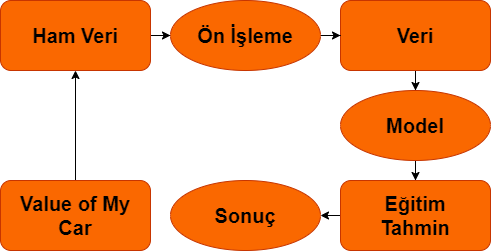
\includegraphics[scale=0.5]{pictures/pic_01.png}&
		\end{tabular}
	\end{center}
	\caption{Value of My Car Akış Diyagramı}
	\label{fig:01}
\end{figure}

Projenin akış diyagramı Şekil \ref{fig:01}'de belirtilmiştir. Makalenin devamında kullanılan algoritmalar ile ilgili bilgiler ve sonuç kısmı bulunmaktadır.

\pagebreak
\section{\textbf{METODLAR}}
\subsection{\textbf{Decision Tree}}

\quad Karar Ağaçları, genellikle regresyon ve sınıflandırma problemlerinde kullanılmaktadır. Ağaç tabanlı algoritmalardan birisi olup karmaşık veri setlerinde kullanılabilir\cite{4}.

\begin{figure}[!h]
	\centering
	\begin{center}
		\begin{tabular}{cc}
			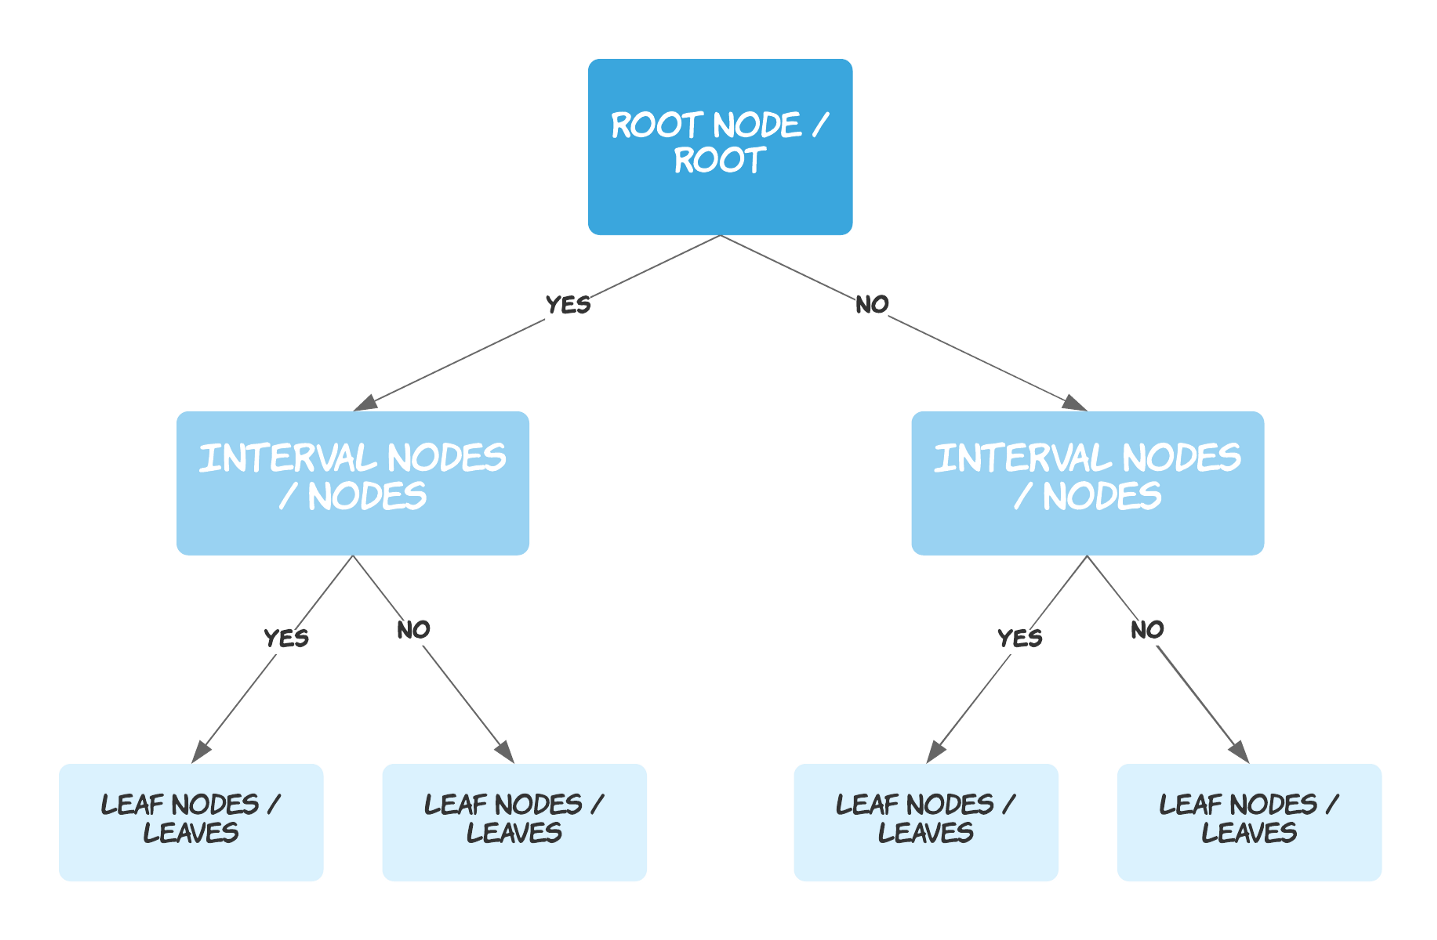
\includegraphics[scale=0.225]{pictures/pic_02.png}&
		\end{tabular}
	\end{center}
	\caption{Decision Tree}
	\label{fig:02}
\end{figure}

\quad Kök (root), Karar Ağaçlarının ilk basamağına(hücresine) verilen isimdir. Problemimizi gözlemlerken, kök kısmındaki koşullar doğrultusunda sınıflandırma yapılır.

\quad Kök hücrelerin altında düğümler (nodes) yer almaktadır. Ele aldığımız her bir gözlem kökler aracılığı ile sınıflandırılır. Düğüm sayısının artma oranıyla doğru orantılı bir şekilde, elimizde bulunan modelin karmaşıklığı da artmaktadır. Bize sonucu veren yapraklardır ve yapraklar ağacın en altında bulunmaktadır\cite{4}.

\quad Kök hücre seçilirken dikkat edilmesi gereken en önemli etken, veri setini iyi açıklayabilmesidir. Köke karar verirken bizim için önemli bazı değerler vardır\cite{4};

\quad Alt kümenin saflık değerine $Gini$ denir ve $T$, $pj$, $j$ sınıfının gerçekleşme olasılığıdır. Elimizdeki her sınıf için ayrı ayrı hesaplanarak çıkan sonuçların karesi alınır. Alınan kareler $1$’den çıkartılır. Bu işlemler sonucunda $(0, 1)$ aralığında bir değer elde edilir. Elde edilen değer $0$’a ne kadar yakınsa o kadar iyi ayrım yapılmıştır\cite{4}.

\quad $Gini$ indexinin formülü Eşitlik \ref{eq:01}'de verilmiştir\cite{15}. Formül değişkenlerinin temsil ettiği veriler de aşağıdaki gibidir;
\begin{itemize}
\item \textbf{$T$:} Tüm veri seti
\item \textbf{$p_{j}$:} Veri setindeki her bir verinin kendinden küçük ve kendinden büyük eleman sayılarına bölümü
\item \textbf{$n$:}  Seçilen verimiz
\end{itemize}

\begin{equation}
\label{eq:01}
\Large Gini(T)=1-\sum_{j=1}^{n}(p_{j})^2
\end{equation}

\pagebreak
\quad Entropy rastgeleliği, belirsizliği ve beklenmeyen durumun ortaya çıkma olasılığını gösterir\cite{5}.  Bu olasılığı $log_{2}$ tabanında yapar\cite{4}.

\begin{equation}
\label{eq:02}
\Large I_{H}=-\sum_{j=1}^{c}p_{j}log_{2}(p_{j})
\end{equation}

\quad Entropi daha dengeli bir ağaç çıkarmaya meyilli iken $Gini$, frekansı fazla olan sınıfı ayrıştırmaya meyillidir.

\subsection{\textbf{Gradient Boosting Regressor}}
\quad Makine öğrenmesi modellerinde tahminlerin doğruluğunu güçlü bir hale getirmek için Gradient Boosting Regressor kullanılır. Yinelemeli olarak çalışan algoritma, karar ağacı tabanlıdır. Gradient Boosting Regressor algoritmasını güçlü kılan faktör; ağaç yapısının, hatayı en az seviyeye düşürecek şekilde olmasıdır\cite{6}.

\quad Gradient Boosting Regressor algoritmasındaki temel amaç, elde edilecek olan maliyet fonksiyonunu en aza düşürebilmek için bulunan parametreleri tekrarlamaktır. Ağaç ekleme işlemi yapılırken kaybı en aza düşürebilmek için gradyan iniş prosedürü kullanılmaktadır \cite{6}.

Gradyan yükseltme üç unsur içerir:

\begin{itemize}
\item Optimize edilmesi beklenen kayıp fonksiyonun(loss) belirlenmesi. 
\item Optimize edilmiş veride belirlenen zayıf öğrenici ile tahmin yapmak. 
\item Loss’u minimum seviyeye indirgemek için zayıf öğrenicilere bir katkı modeli eklenir\cite{7}.
\end{itemize}

\begin{figure}[!h]
	\centering
	\begin{center}
		\begin{tabular}{cc}
			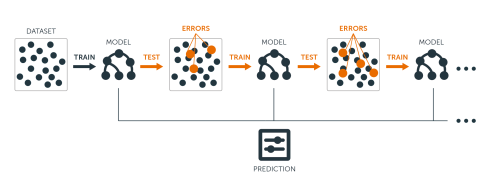
\includegraphics[scale=0.5]{pictures/pic_03.png}&
		\end{tabular}
	\end{center}
	\caption{Gradyan yükseltme algoritması işleyiş süreci\cite{16}}
	\label{fig:03}
\end{figure}

\begin{equation}
\label{eq:03}
\Large Loss^i=\sum_{j=1}^{n}(Y_{j}-F^i(X_{j}))^2
\end{equation}

\pagebreak
\subsection{\textbf{XGB (Extreme Gradient Boosting) Regressor}}

\quad XGBoost, problemleri diğer boosting algoritmalarına göre daha doğru bir yöntemle çözen bir ağaç güçlendirme algoritması olup paralel olarak çalışmaktadır\cite{9}. Tahmin gücünü yükseltmek ve aşırı öğrenmeyi engellemek, algoritmanın temel özelliklerindendir\cite{10}.

\quad XGB’yi tercih etmemizin sebebi, kütüphanesinin; model performansının yüksek ve çalışma süresinin düşük olmasıdır\cite{9}.

\quad XGBoost algoritması kullanılırken öncelikle ilk tahmin (base score) yapılmalıdır. Sonraki adımlarda sonuç herhangi bir sayı olabilir. Çünkü yapılacak işlemler yakınsayarak doğru sonuca ulaşacaktır. Sonraki adımda hataları tahminleyen karar ağacı kurulur. Bu adımdaki amaç hataları öğrenip doğru tahmine yaklaşmaktır. Benzerlik skoru (similarity score) her ağacın her bir dalı için ayrı ayrı hesaplanır. Benzerlik skoru, elimizde bulunan verilerin dallarda ne kadar iyi kategorize olduğunu gösterir\cite{10}.

\begin{equation}
\label{eq:04}
\large Similarity Score=\frac{Sum of Residuals, Squared}{Number of Residuals + \lambda}
\end{equation}

\quad Benzerlik skorlarını hesapladıktan sonra elde ettiğimiz sonuçtan daha iyi bir tahmin yapılıp yapılmayacağını öğrenmek için tüm olasılıklardaki ağaçlar kurulur. Hepsi için ayrı ayrı benzerlik skorları hesaplanır ve hangi ağacın daha etkili yani daha iyi olduğunu tespit etmek için Eşitlik \ref{eq:05}'deki kazanç hesabı yapılır\cite{10}. Yukarıda belirttiğimiz benzerlik skorunun sonucu ile dallar değerlendirilirken, elde ettiğimiz Eşitlik \ref{eq:05}'deki kazanç değeri ile ağacın tamamı değerlendirilmektedir\cite{10}.

\begin{equation}
\label{eq:05}
\begin{matrix} Kazanc=SolBenzerlikSkoru+ \\ SagBenzerlikSkoru-OncekiAgacinBenzerlikSkoru \end{matrix}
\end{equation}

\subsection{\textbf{Random Forest}}
\quad Rastgele Orman Algoritması, denetimli öğrenme algoritması olup hem sınıflandırmada hem de regresyon analizlerinde kullanılır. Aşırı uyumu önler. Random Forest, karar ağaçlarını rastgele bir şekilde oluşturur. İstikrarlı ve doğru bir sonuç tahmini yapabilmek için bunları birleştirir. Rastgele Orman Algoritması’nda; ağaç sayısı ve çıktıları arasında doğrusal bir ilişki vardır. Ağaç sayısı ne kadar arttırılırsa o kadar kesin bir sonuç elde edilir\cite{11}\cite{12}.

\quad Rastgele Orman Algoritması, ağaç büyütme aşamasında, normal durumun üzerine rastgelelik durumunu da kullanmaktadır\cite{12}.
\begin{figure}[!h]
	\centering
	\begin{center}
		\begin{tabular}{cc}
			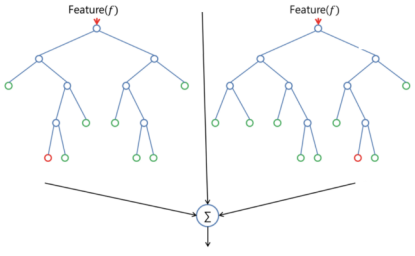
\includegraphics[scale=0.65]{pictures/pic_04.png}&
		\end{tabular}
	\end{center}
	\caption{Random Forest\cite{12}}
	\label{fig:04}
\end{figure}

\pagebreak
\subsection{\textbf{LightGBM Regressor}}
\quad LightGBM, histogram tabanı kullanan bir algoritmadır. Sürekli verileri giriş olarak alır, bu verileri kesikli hale getirir. Bunu yapmasındaki amaç maliyeti azaltmaktır. Karar Ağacı Algoritması’nın bölünmesi ile doğru orantılıdır. Veriyi optimize etmesi, eğitim süresini düşürür ve daha az kaynak kullanılmasını sağlar\cite{13}.

\quad Karar Ağacı Algoritması’nda yaprak ve seviye olarak iki farklı strateji kullanılabilir. Yaprak stratejisinde kayıp oranını azaltan yapraklar üzerinden bölünme işlemi devam eder. Seviye stratejisinde hedeflenen durum ise ağaç büyütülürken dengesini korumaktır. Yaprak stratejisinde hatayı minimize etmek amaçlandığı için, seviye stratejisine göre daha düşük hata oranına sahiptir. Bunun etkilediği durumlardan biri de öğrenme aşamasının hızlanmasıdır. Bu yüzden, boosting algoritmalarının geri kalanından ayrılır. Elimizde bulunan veri sayısı ne kadar çoksa, yaprak stratejisini kullanmak o kadar mantıklı olur. Aşırı öğrenmeye sebebiyet vermemek için veri sayısının az olduğu durumlarda kullanıma uygun değildir. Bu durumda da seviye stratejisi kullanılır\cite{13}.

\begin{figure}[!h]
	\centering
	\begin{center}
		\begin{tabular}{cc}
			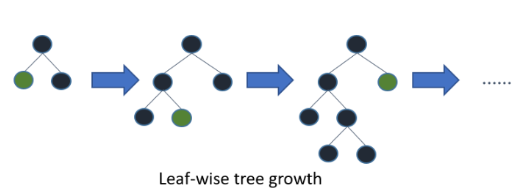
\includegraphics[scale=0.5]{pictures/pic_05.png}&
		\end{tabular}
	\end{center}
	\caption{Yaprak odaklı(leaf wise) strateji\cite{13}}
	\label{fig:05}
\end{figure}

\begin{figure}[!h]
	\centering
	\begin{center}
		\begin{tabular}{cc}
			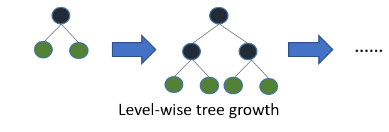
\includegraphics[scale=0.5]{pictures/pic_06.png}&
		\end{tabular}
	\end{center}
	\caption{Seviye odaklı(level wise) strateji\cite{13}}
	\label{fig:06}
\end{figure}
\pagebreak

\subsection{\textbf{CatBoost (Category Boosting) Regressor}}
\quad Gradient Boosting tabanında çalışan, açık kaynaklı bir algoritmadır. Veri hazırlığı süresini düşürdüğü için, boosting algoritmaları arasında önemli bir yere sahiptir. Elinde bulunan boş veriler ile baş edebilir ancak kategorik veriler için kodlamaya ihtiyaç duyar. Yüksek öğrenme hızı, sayısal, kategorik ve metin verileri ile çalışabilmesi en belirgin özelliklerindendir. Ayrıca aşırı öğrenme sorununu ortadan kaldırmak için simetrik ağaç kurar. Aşırı öğrenme durumunun oluşması durumunda, belirlenen özelliklere varmadan önce öğrenme işlemi durdurulur\cite{14}.

\begin{figure}[!h]
	\centering
	\begin{center}
		\begin{tabular}{cc}
			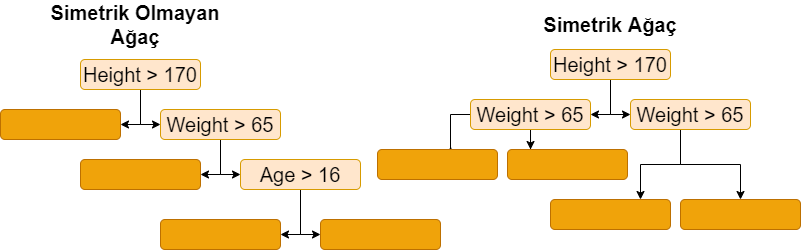
\includegraphics[scale=0.325]{pictures/pic_07.png}&
		\end{tabular}
	\end{center}
	\caption{Simetrik/Simetrik olmayan ağaç}
	\label{fig:07}
\end{figure}

\section{\textbf{SONUÇLAR}}

\quad Veri setindeki veriler \%70 eğitim, \%30 ise test verisi olarak ayrılmıştır. Daha sonra ayrılan veriler, algoritmaların eğitim ve tahmin aşamalarında kullanılmıştır. Bu aşamalar sonucunda elde edilen doğruluk değerlerine Şekil \ref{fig:08}'de, $MSE$ (ortalama kare hatası) değerlerine de Şekil \ref{fig:09}'da yer verilmiştir.

\begin{figure}[!h]
	\centering
	\begin{center}
		\begin{tabular}{cc}
			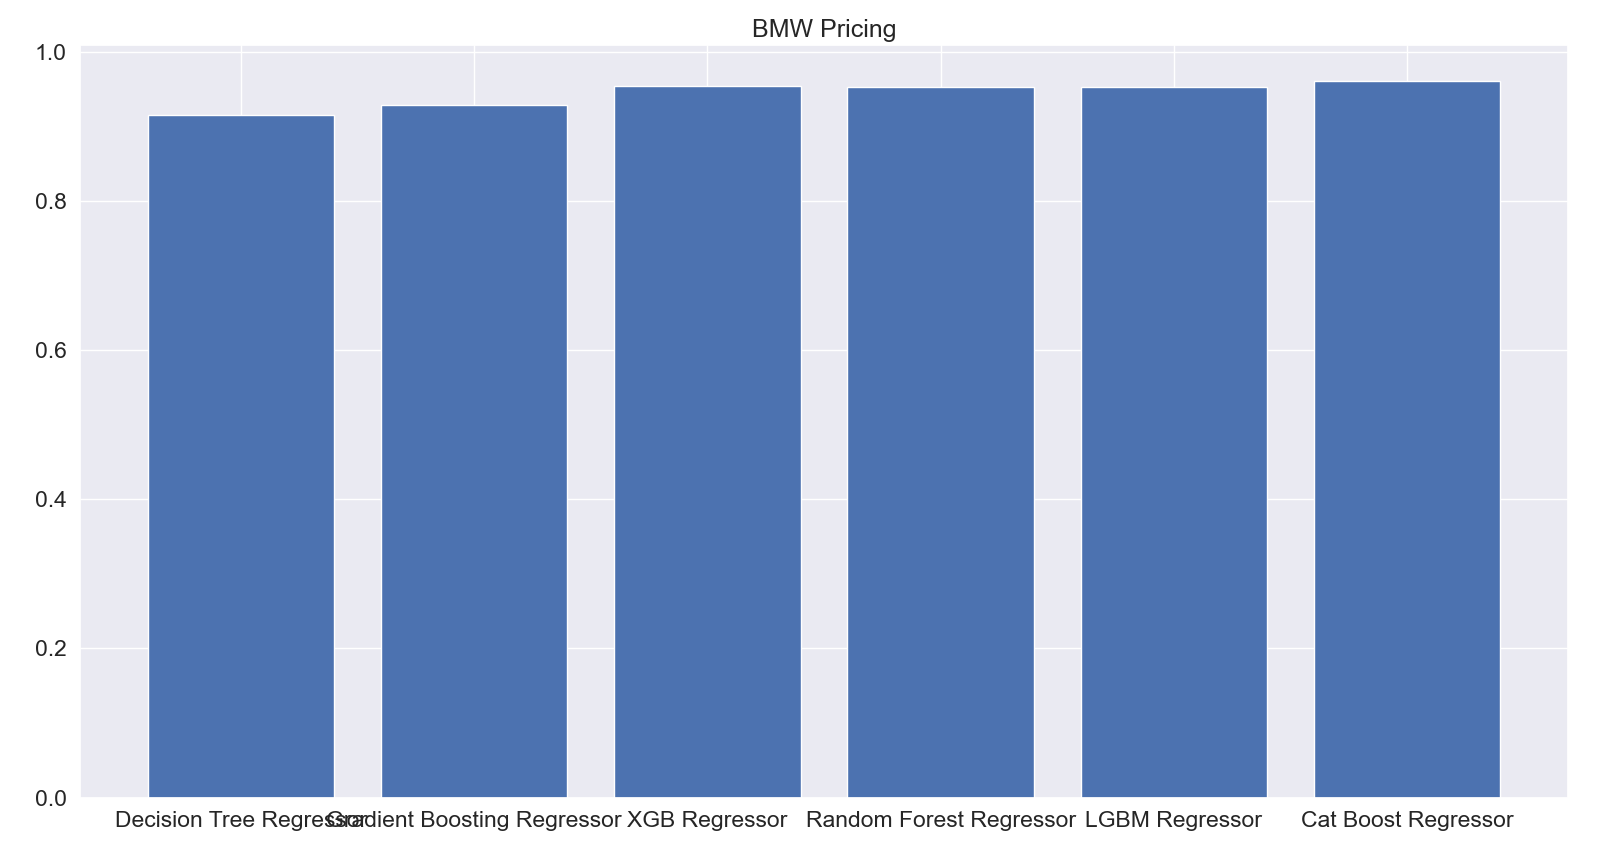
\includegraphics[scale=0.175]{pictures/pic_08.png}&
		\end{tabular}
	\end{center}
	\caption{Tüm Algoritmaların Doğruluk $(r2)$ Değerleri}
	\label{fig:08}
\end{figure}

\begin{figure}[!h]
	\centering
	\begin{center}
		\begin{tabular}{cc}
			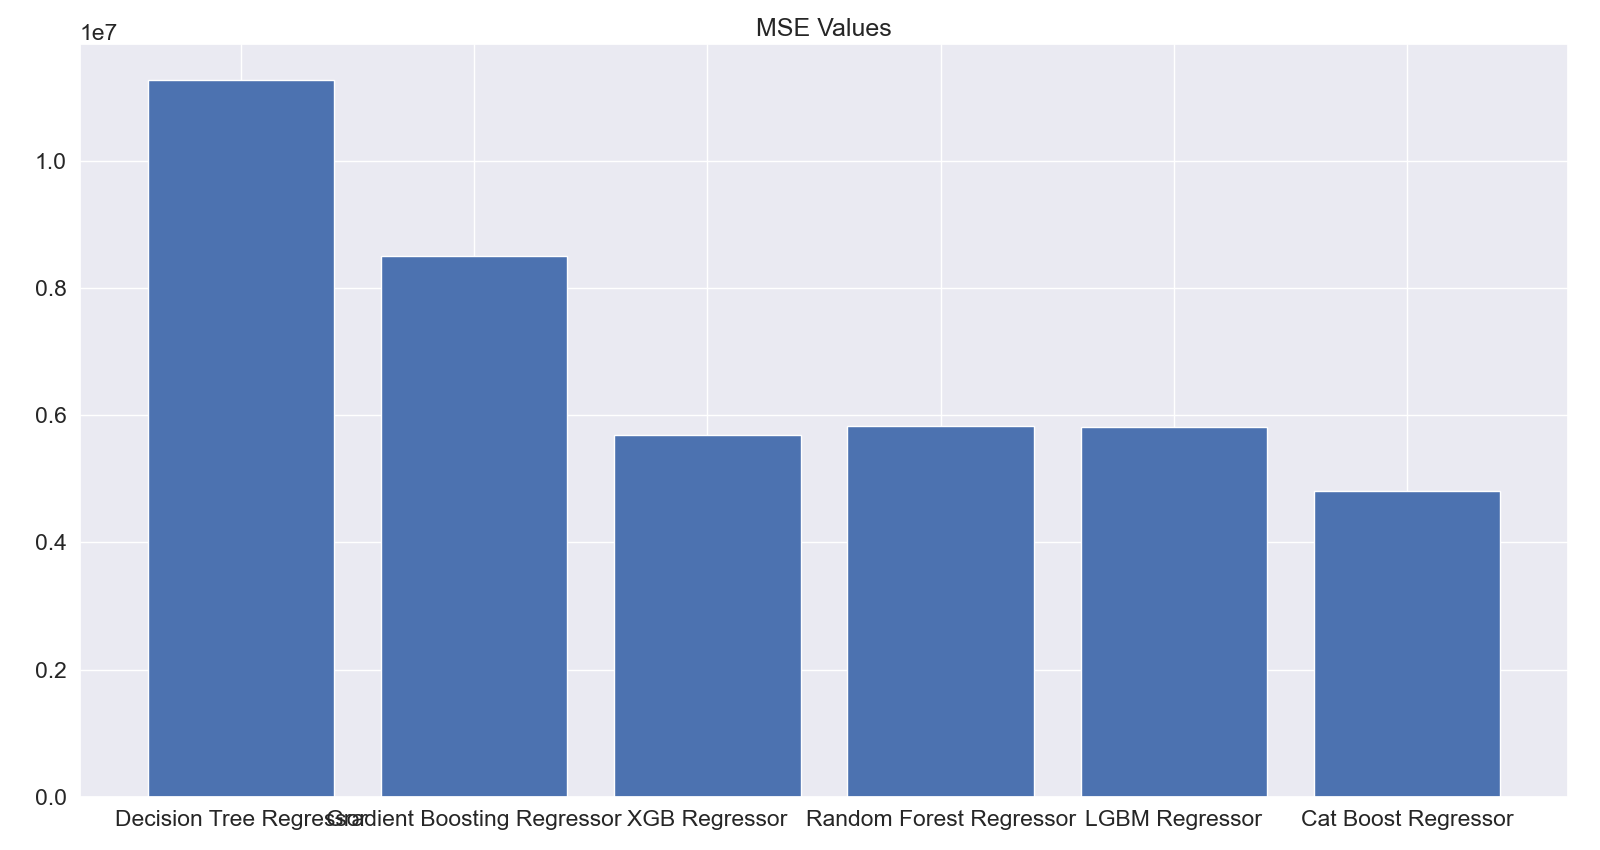
\includegraphics[scale=0.175]{pictures/pic_09.png}&
		\end{tabular}
	\end{center}
	\caption{Tüm Algoritmaların $MSE$ Değerleri}
	\label{fig:09}
\end{figure}

\quad İkinci el araç fiyatlarının tahmin edilebilmesi için "100.000 UK Used Car" \cite{3} veri setindeki "BMW.csv" verisi alındı. DT, GB, XGB, RF, LGBM ve CB regressor algoritmaları kullanılmıştır. Bu algoritmaların $r2$(doğruluk değeri) ve $MSE$(hata değeri) değerleri Tablo \ref{tbl:01}'de yer almaktadır.

\begin{table}[h]
	\centering
	\normalsize
	\begin{tabular}{|l|c|c|c|c|}
		\hline
					& \textbf{r2}	& \textbf{MSE}	\\ \hline
		\textbf{DT}		& 0.9209		& 0.0825		\\ \hline
		\textbf{GB}		& 0.9296		& 0.0657		\\ \hline
		\textbf{XGB}		& 0.9538		& 0.0447		\\ \hline
		\textbf{RF}		& 0.9533		& 0.0453		\\ \hline
		\textbf{LGBM}	& 0.9533		& 0.0449		\\ \hline
		\textbf{CB}		& \textbf{0.9614}	& \textbf{0.0372}	\\ \hline
	\end{tabular}
	\caption{DT, GB, XGB, RF, LGBM ve CB regressor algoritmalarının $r2$ ve $MSE$ degerleri}
	\label{tbl:01}
\end{table}

\quad Tablo \ref{tbl:01}'i incelersek, en yüksek doğruluk değeri$(r2)$nin $\%96.14$ oranıyla CatBoost algoritmasına ait olduğunu görebiliriz. Aynı zamanda en düşük $MSE$(hata) değeri de $0.0372$ oranıyla yine CatBoost algoritmasına aittir. Bu verilerden en düşük doğruluk değerine sahip olan algoritma ise Decision Tree$(\%92.09)$ algoritmasıdır. $r2$ ve $MSE$ değerlerinin arasındaki ters orantıdan dolayı, en yüksek $MSE$ değeri yine Decision Tree$(0.0825)$ algoritmasına aittir. Diğer algoritmaların $r2$ ve $MSE$ değerleri de Tablo \ref{tbl:01} üzerinden incelenebilir.

\subsection{\textbf{Cross-Validation (Çapraz Doğrulama)}}
\quad Cross-Validation, makine öğrenmesi algoritmalarının tâbi tutulabileceği bir fonksiyondur. Modelin eğitiminde kullanılacak olan veriyi, her seferinde farklı kısımlardan bölerek $(train-test)$ optimum sonucu bulmayı amaçlar.

\quad Regresyon algoritmaları birer kez eğitilmiştir. Bu eğitimlerin sonuçları da Tablo \ref{tbl:01}'de belirtilmiştir. DT, GB, XGB, RF, LGBM ve CB algoritmaları \textbf{Cross-Validation} metoduyla 30 kez rastgele olacak şekilde çalıştırılmış ve sonuçları Şekil \ref{fig:10}, \ref{fig:11}, \ref{fig:12}, \ref{fig:13}, \ref{fig:14} ve \ref{fig:15}'de verilmiştir.

\begin{figure}[!h]
	\centering
	\begin{center}
		\begin{tabular}{cc}
			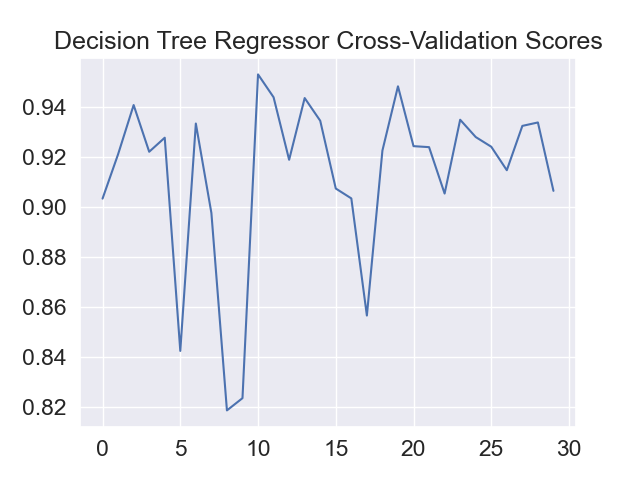
\includegraphics[scale=0.5]{pictures/pic_10.png}&
		\end{tabular}
	\end{center}
	\caption{Decision Tree Regressor Cross-Validation}
	\label{fig:10}
\end{figure}
\pagebreak
\begin{figure}[!h]
	\centering
	\begin{center}
		\begin{tabular}{cc}
			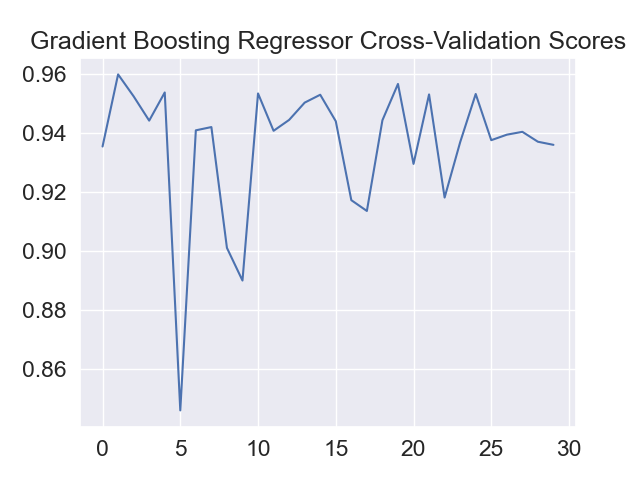
\includegraphics[scale=0.5]{pictures/pic_11.png}&
		\end{tabular}
	\end{center}
	\caption{Gradient Boost Regressor Cross-Validation}
	\label{fig:11}
\end{figure}

\begin{figure}[!h]
	\centering
	\begin{center}
		\begin{tabular}{cc}
			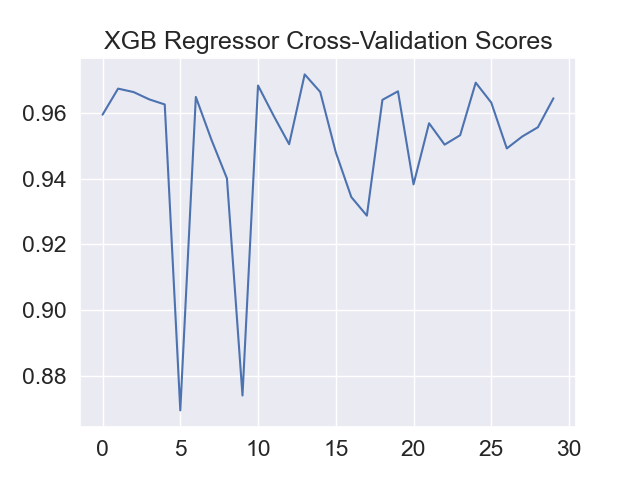
\includegraphics[scale=0.5]{pictures/pic_12.png}&
		\end{tabular}
	\end{center}
	\caption{XGB Regressor Cross-Validation}
	\label{fig:12}
\end{figure}

\begin{figure}[!h]
	\centering
	\begin{center}
		\begin{tabular}{cc}
			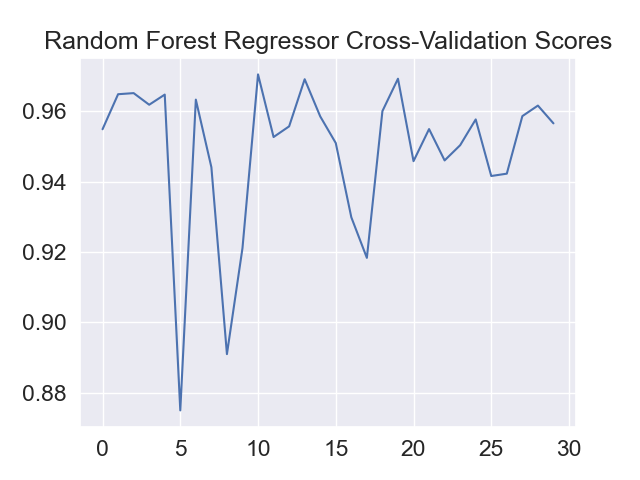
\includegraphics[scale=0.5]{pictures/pic_13.png}&
		\end{tabular}
	\end{center}
	\caption{Random Forest Regressor Cross-Validation}
	\label{fig:13}
\end{figure}
\pagebreak
\begin{figure}[!h]
	\centering
	\begin{center}
		\begin{tabular}{cc}
			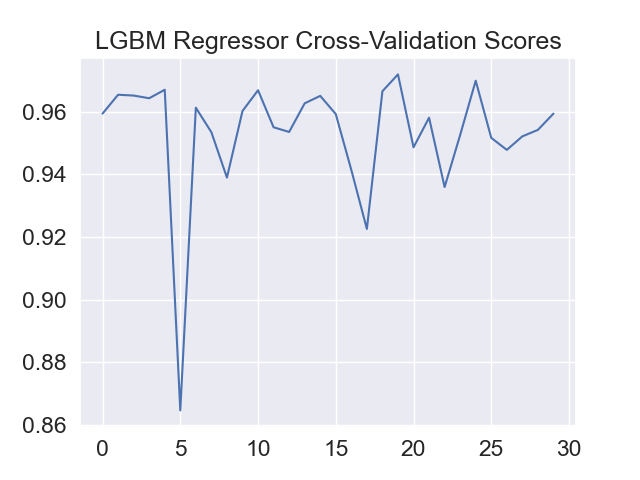
\includegraphics[scale=0.5]{pictures/pic_14.png}&
		\end{tabular}
	\end{center}
	\caption{LGBM Regressor Cross-Validation}
	\label{fig:14}
\end{figure}

\begin{figure}[!h]
	\centering
	\begin{center}
		\begin{tabular}{cc}
			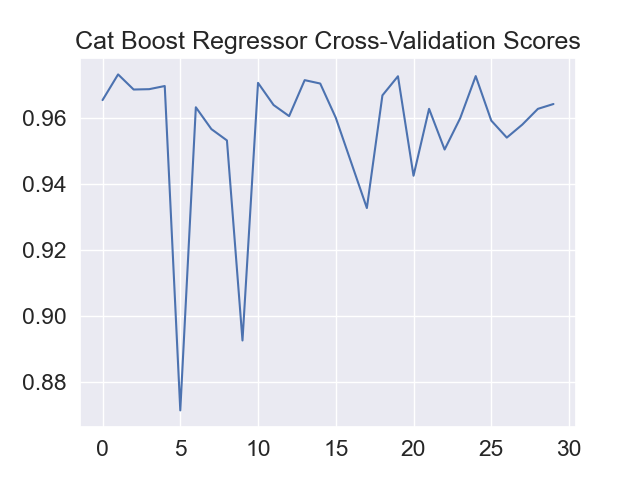
\includegraphics[scale=0.5]{pictures/pic_15.png}&
		\end{tabular}
	\end{center}
	\caption{CatBoost Regressor Cross-Validation}
	\label{fig:15}
\end{figure}

\quad Bu algoritmaların Cross-Validation sonuçlarının ortalamaları Şekil \ref{fig:16}'daki gibidir. Bu değerler aynı zamanda Tablo \ref{tbl:02}'de de sayısal olarak yer almaktadır.

\begin{figure}[!h]
	\centering
	\begin{center}
		\begin{tabular}{cc}
			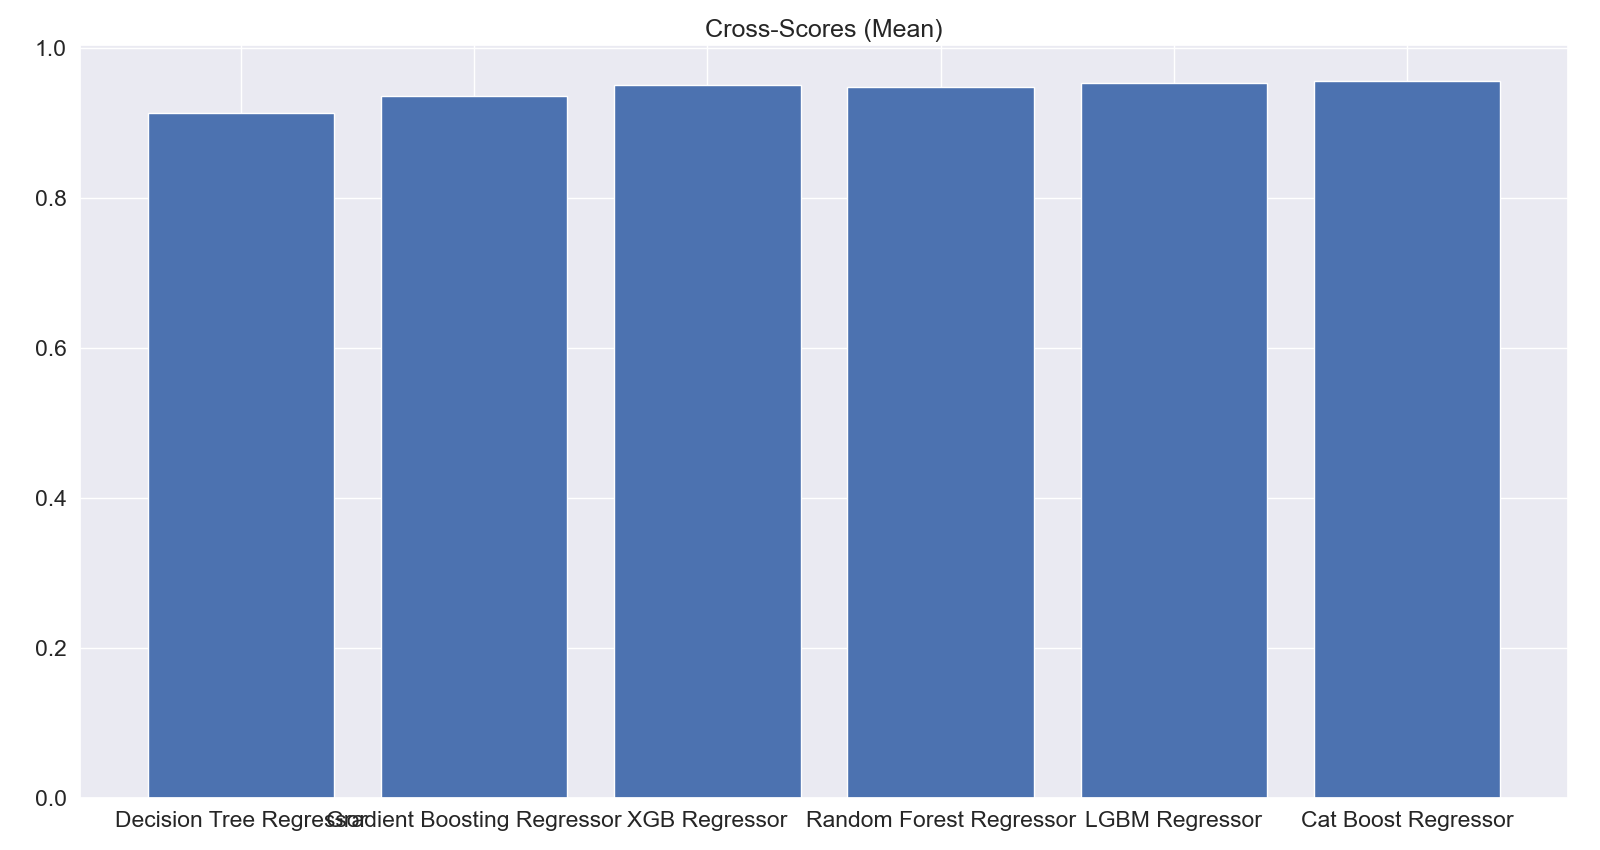
\includegraphics[scale=0.2]{pictures/pic_16.png}&
		\end{tabular}
	\end{center}
	\caption{Cross-Validation Ortalama(Mean) Değerleri}
	\label{fig:16}
\end{figure}
\pagebreak
\begin{table}[h]
	\centering
	\normalsize
	\begin{tabular}{|l|c|c|c|c|}
		\hline
					& \textbf{Cross-Validation Score(mean)}	\\ \hline
		\textbf{DT}		& 0.9160		\\ \hline
		\textbf{GB}		& 0.9356		\\ \hline
		\textbf{XGB}		& 0.9512		\\ \hline
		\textbf{RF}		& 0.9485		\\ \hline
		\textbf{LGBM}	& 0.9531		\\ \hline
		\textbf{CB}		& \textbf{0.9562}	\\ \hline
	\end{tabular}
	\caption{DT, GB, XGB, RF, LGBM ve CB algoritmalarının Cross-Validation sonuçlarının ortalama(mean) degerleri}
	\label{tbl:02}
\end{table}

\quad Tablo \ref{tbl:02}'yi incelersek, en yüksek doğruluk değerinin $\%95.62$ oranıyla CatBoost algoritmasına ait olduğu görülebilir. Bu verilerden en düşük doğruluk değerine sahip olan algoritma ise Decision Tree$(\%91.60)$ algoritmasıdır. Diğer algoritmaların Cross-Validation sonuçlarının ortalama değerlerini de Tablo \ref{tbl:02} üzerinde incelenebilir.

\subsection{\textbf{Valid Data-Pred Data$(Diff)$}}

\quad Şekil \ref{fig:17}, \ref{fig:18}, \ref{fig:19}, \ref{fig:20}, \ref{fig:21} ve \ref{fig:22}'de de gösterildiği gibi; gerçek $(valid)$ verilerimiz turuncu, algoritmanın tahmin $(predict)$ değerleri ise mavi hatlarla belirtilmiştir. Bu grafikleri oluşturmaktaki amaç; tahmin verisinin gerçek veriden ne kadar saptığını(uzaklaştığını/saptığını) görmektir.
\begin{figure}[!h]
	\centering
	\begin{center}
		\begin{tabular}{cc}
			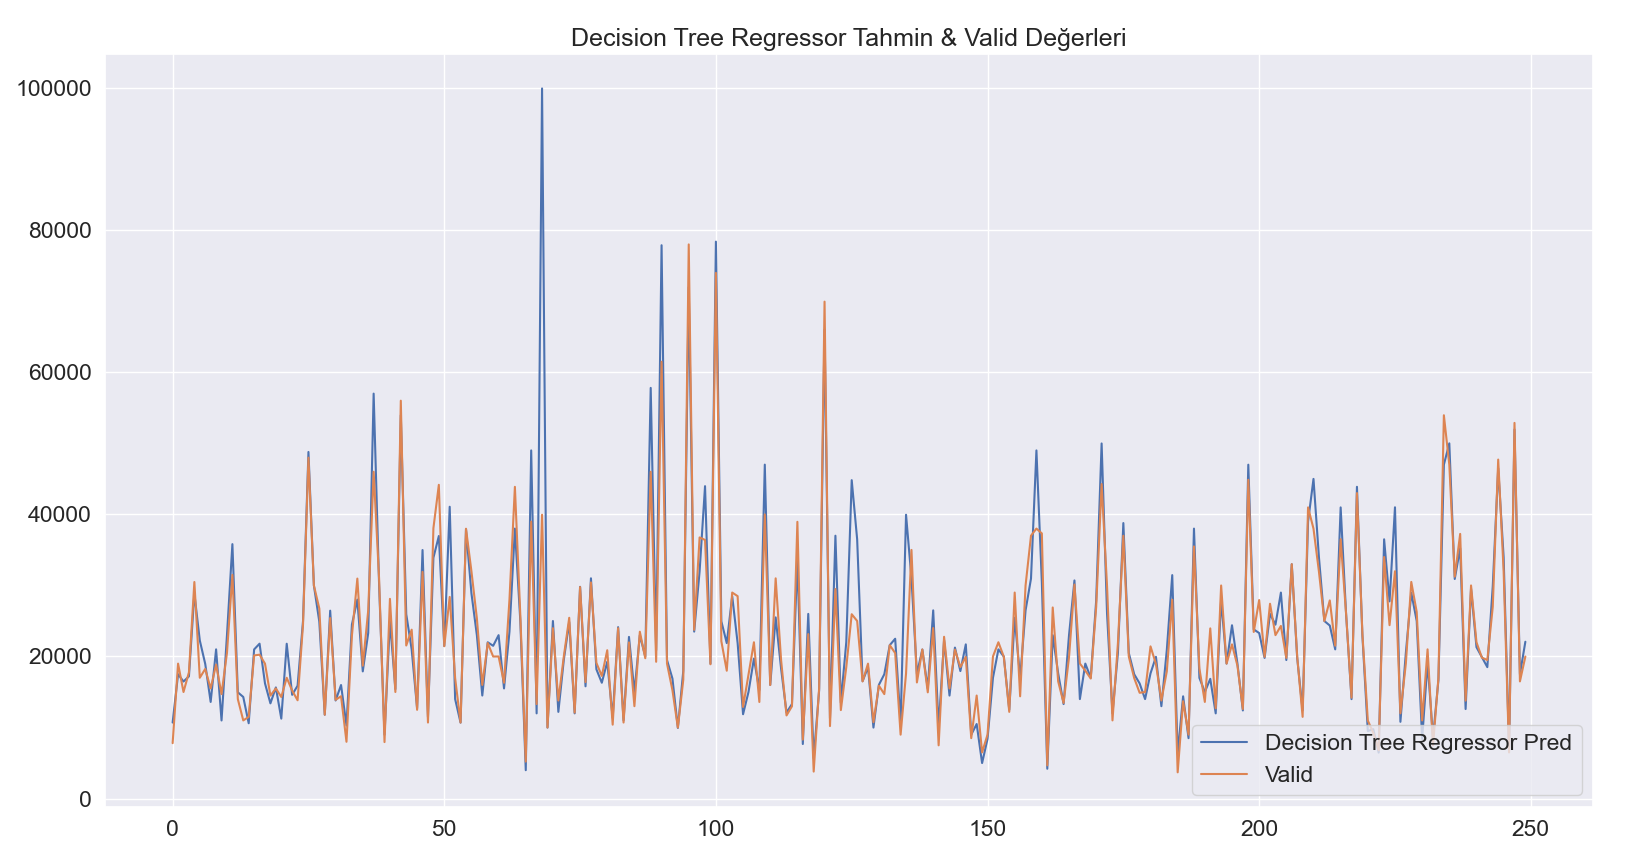
\includegraphics[scale=0.2]{pictures/pic_17.png}&
		\end{tabular}
	\end{center}
	\caption{Decision Tree Regressor Tahmin \& Valid Değerleri}
	\label{fig:17}
\end{figure}

\begin{figure}[!h]
	\centering
	\begin{center}
		\begin{tabular}{cc}
			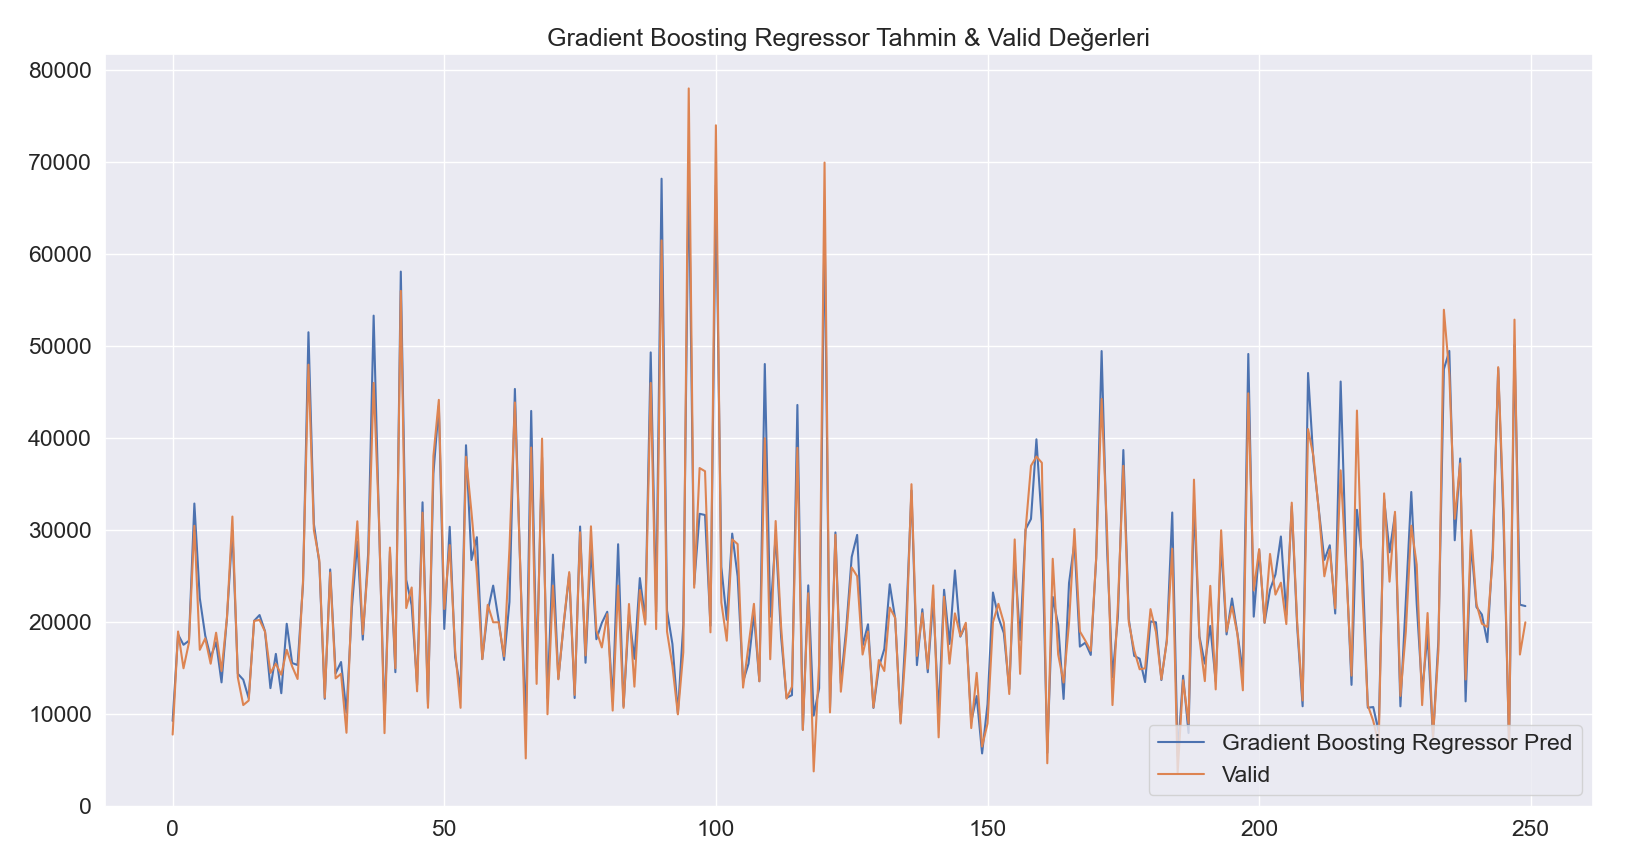
\includegraphics[scale=0.2]{pictures/pic_18.png}&
		\end{tabular}
	\end{center}
	\caption{Gradient Boosting Regressor Tahmin \& Valid Değerleri}
	\label{fig:18}
\end{figure}
\pagebreak
\begin{figure}[!h]
	\centering
	\begin{center}
		\begin{tabular}{cc}
			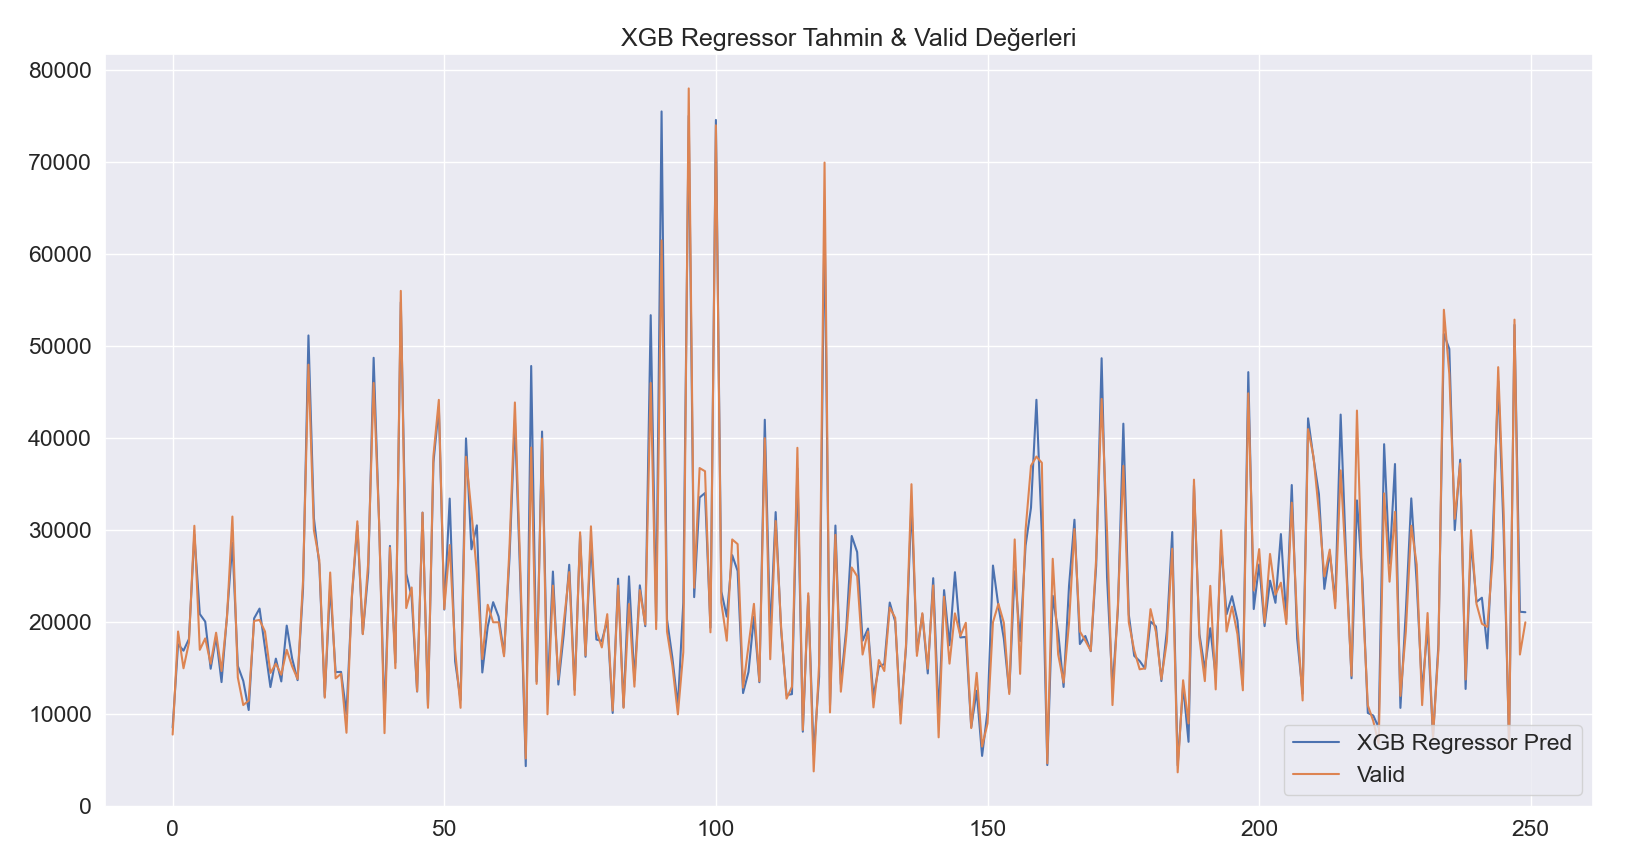
\includegraphics[scale=0.18]{pictures/pic_19.png}&
		\end{tabular}
	\end{center}
	\caption{XGB Regressor Tahmin \& Valid Değerleri}
	\label{fig:19}
\end{figure}

\begin{figure}[!h]
	\centering
	\begin{center}
		\begin{tabular}{cc}
			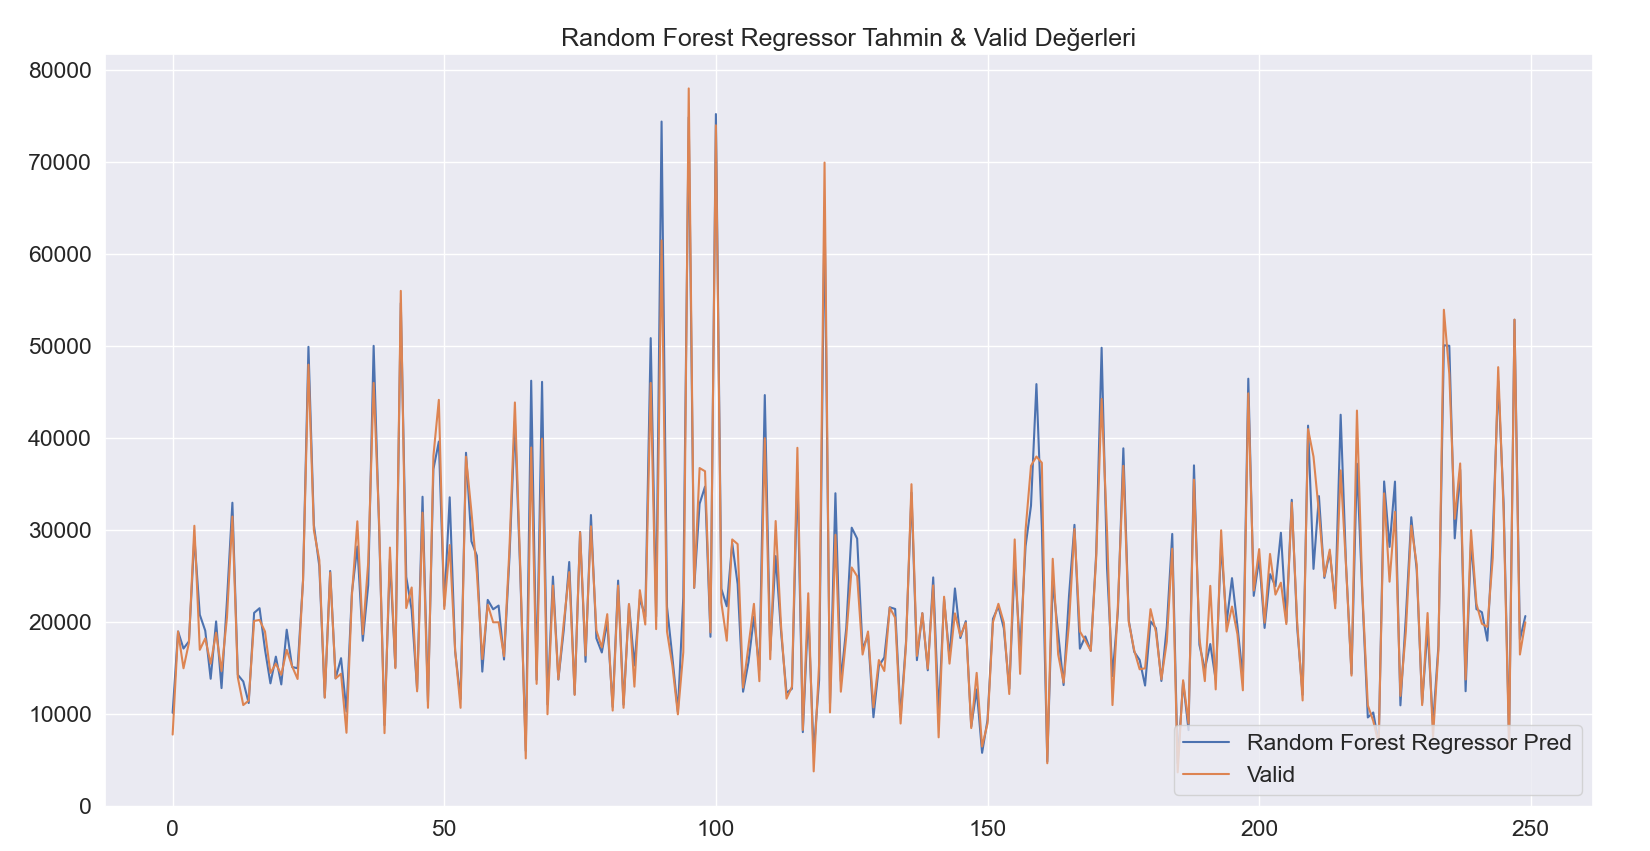
\includegraphics[scale=0.18]{pictures/pic_20.png}&
		\end{tabular}
	\end{center}
	\caption{Random Forest Regressor Tahmin \& Valid Değerleri}
	\label{fig:20}
\end{figure}

\begin{figure}[!h]
	\centering
	\begin{center}
		\begin{tabular}{cc}
			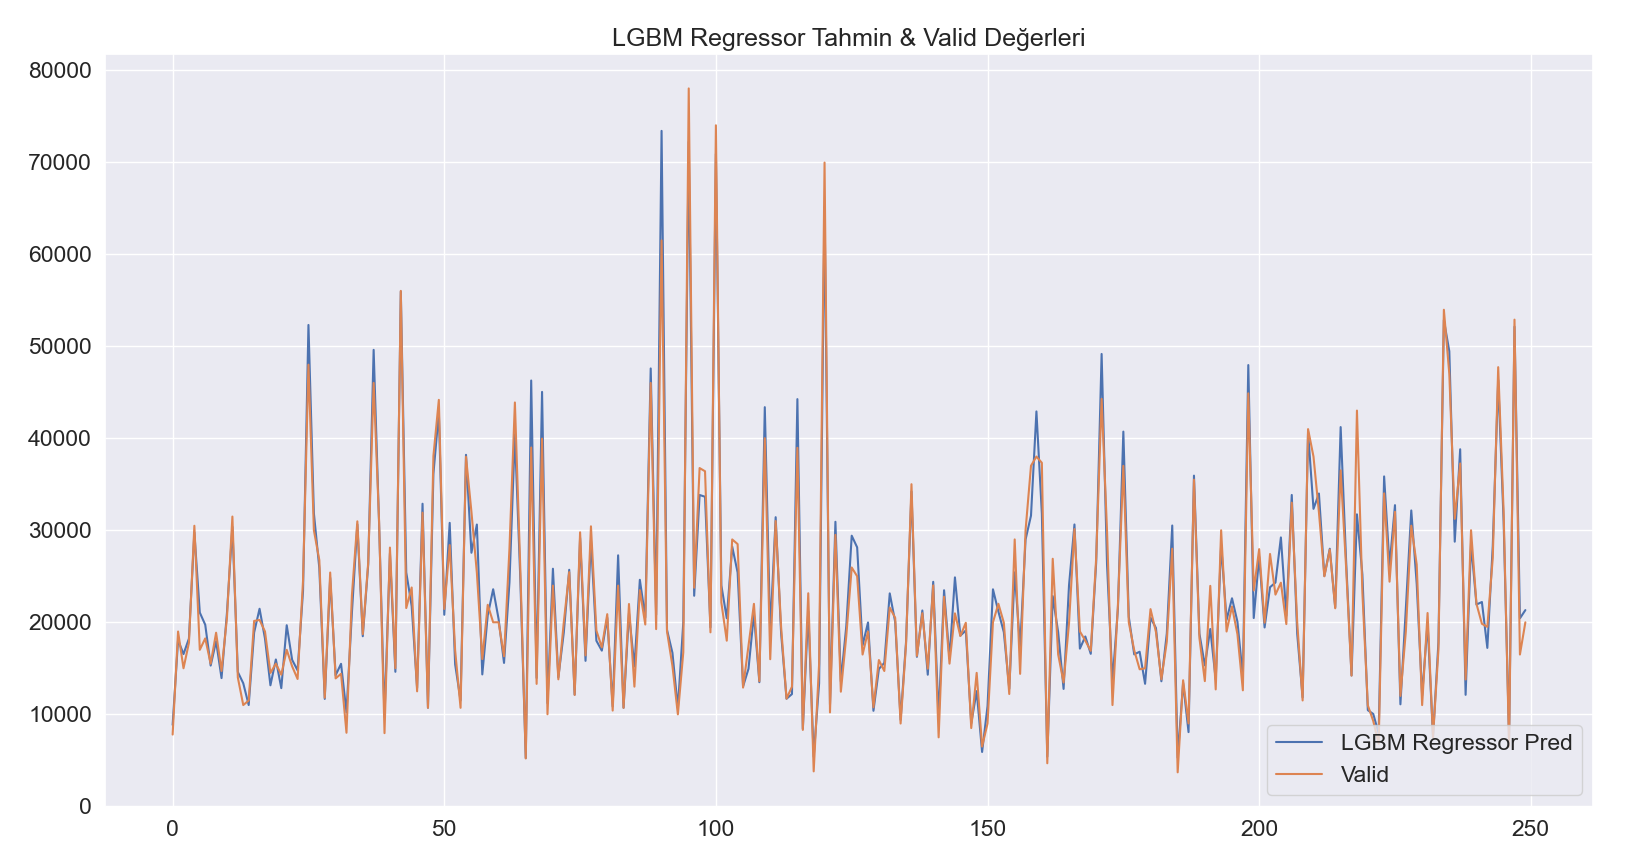
\includegraphics[scale=0.18]{pictures/pic_21.png}&
		\end{tabular}
	\end{center}
	\caption{LGBM Regressor Tahmin \& Valid Değerleri}
	\label{fig:21}
\end{figure}

\begin{figure}[!h]
	\centering
	\begin{center}
		\begin{tabular}{cc}
			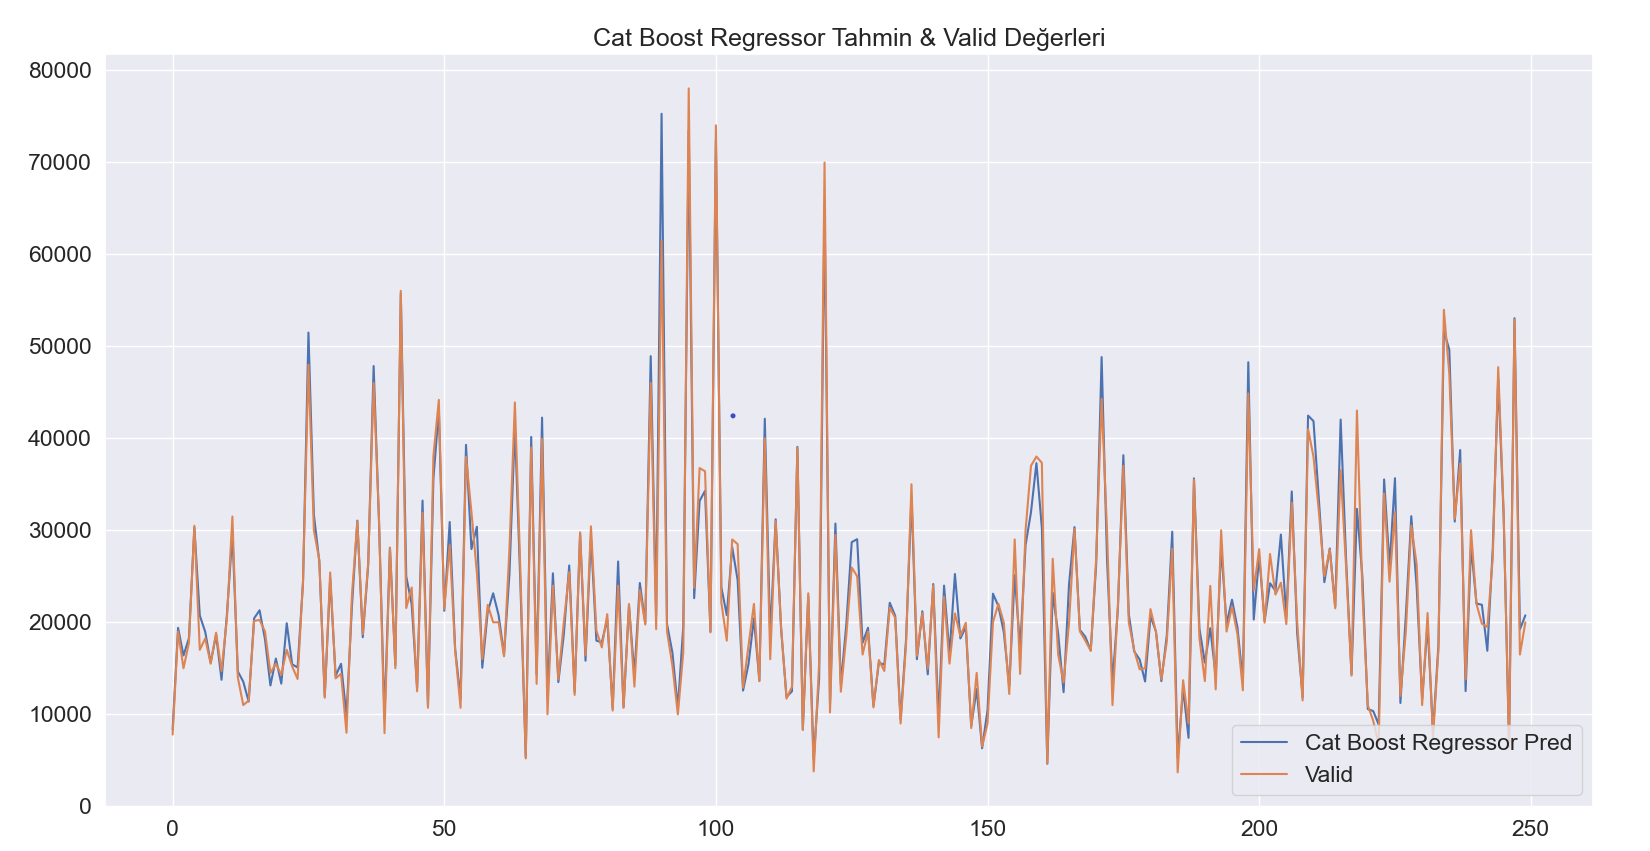
\includegraphics[scale=0.18]{pictures/pic_22.png}&
		\end{tabular}
	\end{center}
	\caption{CatBoost Regressor Tahmin \& Valid Değerleri}
	\label{fig:22}
\end{figure}
\pagebreak


\section{\textbf{SONUÇ}}

\quad Projede kullanılan veri seti sayesinde ikinci el araçların, değerinin altında veya üzerinde bir fiyata satılması yerine, olması gereken bir fiyatta satılmasını sağlamak için; yapay zekâ algoritmaları kullanılarak fiyat tahmini yapılmaya çalışıldı. Algoritmaları, makalenin önceki başlıklarında da anlatıldığı gibi çeşitli işlemlere tâbi tutularak, bazı sonuçlar elde edildi. Çıkan sonuçlar karşılaştırıldı ve en iyi algoritma bulunmaya çalışıldı. Eldeki veri setiyle en uyumlu çalışan algoritma bulundu ve raporlandı. Eğitim sonuçlarını daha yüksek oranlara taşıyabilmek için veri seti optimize edilebilir, gerekli öznitelikler eklenebilir veya gereksiz olanlar çıkartılabilir. Bu sayede daha doğru bir tahminleme işlemi yapılabilir.

\begin{figure}[!h]
	\centering
	\begin{center}
		\begin{tabular}{cc}
			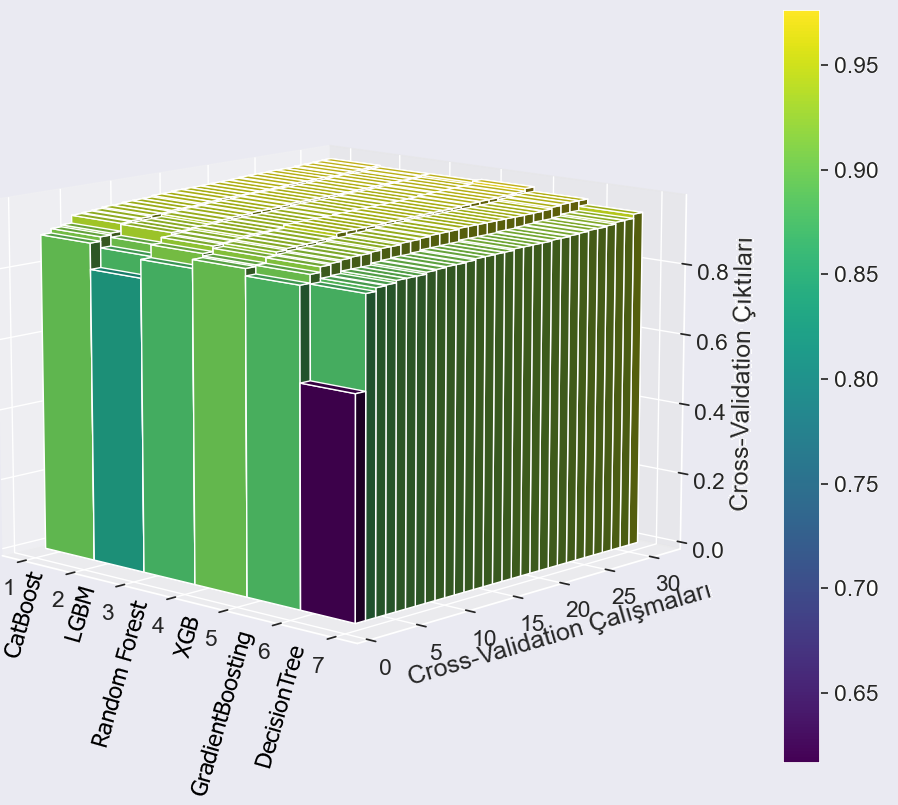
\includegraphics[scale=0.35]{pictures/pic_23.png}&
		\end{tabular}
	\end{center}
	\caption{Algoritmaların Cross-Validation Sonuçları (3D Grafik)}
	\label{fig:23}
\end{figure}
\quad $X$ eksenine bakıldığı zaman algoritmaları, $Y$ eksenine bakıldığı zaman algoritmaların çalışma sayıları görülebilir. Daha sonradan 3. boyuta ise bu çalışmaların skorları $Z$ ekseni olarak eklendi ve Şekil \ref{fig:23}'deki 3D grafik elde edildi. Algoritmalar ve çalışma skorları, kendi arasında sıralı olduğu için, sütunlara çapraz açıdan bakıldığında en verimli algoritmanın en yüksekte kaldığı görülebilir.

\quad Aynı veri setini kullanan başka bir kullanıcının verilerinin\cite{17} çıktıları da Tablo \ref{tbl:03}'te yer almaktadır. Bu veriler incelendiği zaman bazı noktalarda daha yüksek, bazı noktalarda daha düşük doğruluk $(r2)$ değeri elde edildiği görülebilir. Ancak $MSE$ değeri incelendiği zaman, projemizin daha düşük hata değerine sahip olduğu görülebilir. Bunun sebebi, veri setinin $zscore$ işlemine tâbi tutulmuş olmasıdır.

\begin{table}[h]
	\centering
	
\begin{tabular}{|c|cc|cc|}
\hline
\multirow{2}{*}{}          & \multicolumn{2}{c|}{\textbf{Mevcut Proje}}      & \multicolumn{2}{c|}{\textbf{rajan1002}}         \\ \cline{2-5} 
                           & \multicolumn{1}{c|}{\textbf{R2}} & \textbf{MSE} & \multicolumn{1}{c|}{\textbf{R2}} & \textbf{MSE} \\ \hline
\textbf{Random Forest}     & \multicolumn{1}{c|}{0.9533}      & \textbf{0.0453}       & \multicolumn{1}{c|}{0.9508}      & 0.1180       \\ \hline
\textbf{Gradient Boosting} & \multicolumn{1}{c|}{0.9296}      & 0.0657       & \multicolumn{1}{c|}{0.9479}      & 0.1214       \\ \hline
\textbf{XGB Regressor}     & \multicolumn{1}{c|}{\textbf{0.9538}}      & 0.0447       & \multicolumn{1}{c|}{\textbf{0.9562}}      & \textbf{0.1113}       \\ \hline
\end{tabular}
\caption{\textbf{rajan1002}'nin eğitim sonuçları\cite{17} ile karşılaştırma}
	\label{tbl:03}
\end{table}
\newpage
%%%%%%%%%%%%%%%%%%%%
\newpage
\begin{thebibliography}{17}

\bibitem{1}
DergiPark - İkinci El Otomobil Talep Fiyatının Regresyon Analizi
\\\texttt{\href{https://dergipark.org.tr/tr/download/article-file/431769}{\nolinkurl{dergipark.org.tr/article-file/431769}}}

\bibitem{2}
IjcaOnline - Vehicle Price Prediction
\\\texttt{\href{https://www.ijcaonline.org/archives/volume167/number9/noor-2017-ijca-914373.pdf}{\nolinkurl{ijcaonline.org/archives/noor-2017-ijca-914373}}}

\bibitem{3}
Kaggle - 100.000 UK Used Car Data Set
\\\texttt{\href{https://www.kaggle.com/adityadesai13/used-car-dataset-ford-and-mercedes?select=bmw.csv}{\nolinkurl{kaggle.com/adityadesai13/used-car-dataset-bmw}}}

\bibitem{4}
Medium - Karar Ağaçları
\\\texttt{\href{https://medium.com/deep-learning-turkiye/karar-ağaçları-makine-öğrenmesi-serisi-3-a03f3ff00ba5}{\nolinkurl{medium.com/deep-learning/karar-ağaçlari}}}

\bibitem{5}
Başkent - Karar Ağacı
\\\texttt{\href{http://mail.baskent.edu.tr/~20410964/DM_8.pdf}{\nolinkurl{baskent.edu.tr/20410964/DM_8.pdf}}}

\bibitem{6}
Data Science - Boosting Algoritmaları
\\\texttt{\href{https://www.datasciencearth.com/boosting-algoritmalari/}{\nolinkurl{datasciencearth.com/boosting-algoritmalari}}}

\bibitem{7}
Tevfik Bulut - Gradyan Yükseltme Algoritması
\\\texttt{\href{https://tevfikbulut.com/2020/06/27/topluluk-ogrenme-algoritmalarindan-gradyan-yukseltme-algoritmasi-ile-gogus-kanserinin-tahmini-uzerine-bir-vaka-calismasi-a-case-study-on-the-prediction-of-breast-cancer-using-gradient-boosting-algori/}{\nolinkurl{tevfikbulut.com/prediction-of-breast-cancer}}}

\bibitem{8}
OpenGenus - Boosting Algorithms
\\\texttt{\href{https://iq.opengenus.org/types-of-boosting-algorithms/}{\nolinkurl{opengenus.org/types-of-boosting-algorithms}}}

\bibitem{9}
OpenGenus - XGBoost
\\\texttt{\href{https://iq.opengenus.org/xgboost/}{\nolinkurl{opengenus.org/xgboost}}}

\bibitem{10}
Veri Bilimi Okulu  - XGBoost Nasıl Çalışır
\\\texttt{\href{https://www.veribilimiokulu.com/xgboost-nasil-calisir/}{\nolinkurl{veribilimiokulu.com/xgboost-nasil-calisir}}}

\bibitem{11}
Medium - Rastgele Orman Algoritması
\\\texttt{\href{https://medium.com/@cemthecebi/rastgele-orman-algoritması-1600ca4f4784}{\nolinkurl{medium.com/@cemthecebi/rastgele-orman}}}

\bibitem{12}
DevHunter - Rastgele Orman Algoritması
\\\texttt{\href{https://devhunteryz.wordpress.com/2018/09/20/rastgele-ormanrandom-forest-algoritmasi/comment-page-1/}{\nolinkurl{devhunteryz.wordpress.com/random-forest}}}

\bibitem{13}
Veri Bilimi Okulu - LightGBM
\\\texttt{\href{https://www.veribilimiokulu.com/lightgbm/}{\nolinkurl{veribilimiokulu.com/lightgbm}}}

\bibitem{14}
Veri Bilimi Okulu - CatBoost Nedir
\\\texttt{\href{https://www.veribilimiokulu.com/catboost-nedir-diger-boosting-algoritmalarindan-farki-nelerdir/}{\nolinkurl{veribilimiokulu.com/catboost}}}

\bibitem{15}
SlideShare - Random Forest
\\\texttt{\href{https://www.slideshare.net/SezerFidanc/random-forest-algoritmas}{\nolinkurl{slideshare.net/SezerFidanc/random-forest-algoritmasi}}}

\bibitem{16}
BradleyBoehmke - GBM
\\\texttt{\href{https://bradleyboehmke.github.io/HOML/gbm.html}{\nolinkurl{bradleyboehmke.github.io/gbm.html}}}

\bibitem{17}
Kaggle - Used Car Price Prediction
\\\texttt{\href{https://www.kaggle.com/rajan1002/used-car-price-prediction-r2-0-956}{\nolinkurl{kaggle.com/rajan1002/used-car-price-prediction}}}

\end{thebibliography}

\end{document}